% fig:paired-lookup -- float body for Sections/04d-baselines.tex (sec:res-lookup),
% to be placed with the closing \begin{claim} block. \input this, or paste it.
% The graphic is drawn at 174mm by thesis_v2/figs/paired-lookup.py; NO width= key,
% so it is placed at scale 1.0 and its type prints at the sizes it was set in.
\begin{figure}[htbp]
\begin{fullwidth}
\centering
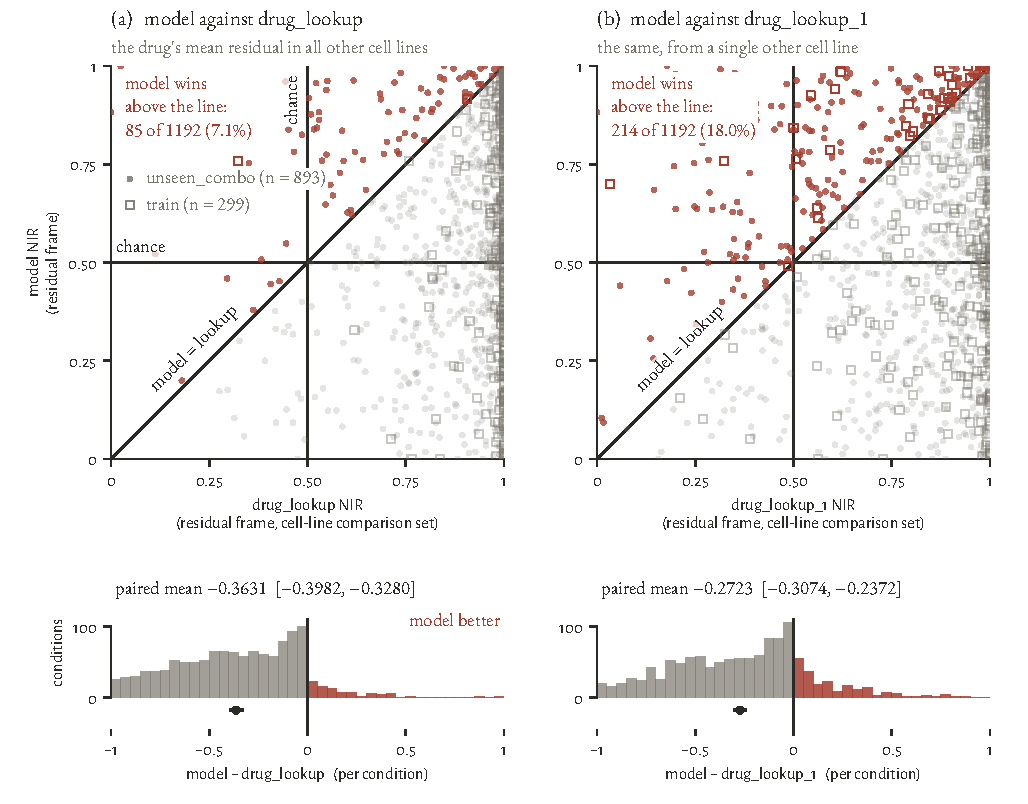
\includegraphics{fig-paired-lookup}
\caption[The paired distribution behind the headline gap]{\captiontitle{The gap is not
an average over a mixed population: the model is above the identity line on
$7.1\%$ of conditions against \texttt{drug\_lookup}, and on $18.0\%$ against the
single-cell-line lookup.} Every mark is one of the
$\num{1192}$ conditions of the common support --- the conditions on which a
training-only lookup exists --- and both axes are $\NIR$ in the \Rframe{} frame,
comparison set other drugs in the same cell line. On this support the model
scores $0.549$ and the within-well split-half precision reference $0.857$;
$\num{1394}$-condition figures quoted elsewhere ($0.537$, $0.854$) are a
different population and are not combined with these. (a) Against
\texttt{drug\_lookup}, the drug's mean residual in all other cell lines: the
model is above the identity line on $85$ of $\num{1192}$ conditions, $7.1\%$.
(b) Against \texttt{drug\_lookup\_1}, the same quantity from a single other cell
line, which scores $0.822$ pooled: $214$ of $\num{1192}$, $18.0\%$. Marker shape
gives the split, $\num{299}$ \texttt{train} and \needsaudit{893}
\texttt{unseen\_combo}; no \texttt{unseen\_drug} condition appears, because no
training lookup exists for a drug held out of training, and that regime is
therefore not addressed by this figure at all. The lower panels are the
per-condition paired difference on a shared count axis, with the paired mean
drawn below the counts as a point and bar, the bar a $95\%$ bootstrap interval
clustered two-way on cell line and well: \ci{-0.3631}{-0.3982}{-0.3280} in (a) and
\ci{-0.2723}{-0.3074}{-0.2372} in (b). The win counts are counts over conditions
and carry no interval; ties ($23$ and $28$ conditions) count as not a win. The
$0.50$ rules are chance on both axes, labelled once in (a).}
\label{fig:paired-lookup}
\end{fullwidth}
\end{figure}
